\documentclass[tikz, border=25pt]{standalone}
\usepackage{xcolor}
\usepackage{helvet}
\renewcommand{\familydefault}{\sfdefault}
\usepackage{amsmath}
\usetikzlibrary{shapes.geometric, arrows.meta, positioning, fit, backgrounds, calc}

\definecolor{phase1bg}{HTML}{F0F6FF}
\definecolor{phase1border}{HTML}{2563EB}
\definecolor{boxbg}{HTML}{D9E8FD}
\definecolor{boxborder}{HTML}{3B82F6}
\definecolor{arrowblue}{HTML}{2563EB}
\definecolor{textcolor}{HTML}{0F172A}

\hyphenpenalty=10000
\exhyphenpenalty=10000

\tikzset{
  stepbox/.style={
    draw=boxborder,
    fill=boxbg,
    line width=1.8pt,
    rounded corners=12pt,
    align=center,
    text=textcolor,
    font=\sffamily\bfseries\Large,
    inner sep=14pt,
    text width=11.5cm,
    minimum height=1.6cm
  },
  flowarrow/.style={
    -{Stealth[length=15pt, width=12pt]},
    line width=3.8pt,
    color=arrowblue,
    shorten >= 6pt,
    shorten <= 6pt
  },
  container/.style={
    draw=phase1border,
    fill=phase1bg,
    line width=2.8pt,
    rounded corners=22pt,
    inner sep=24pt
  }
}

\begin{document}
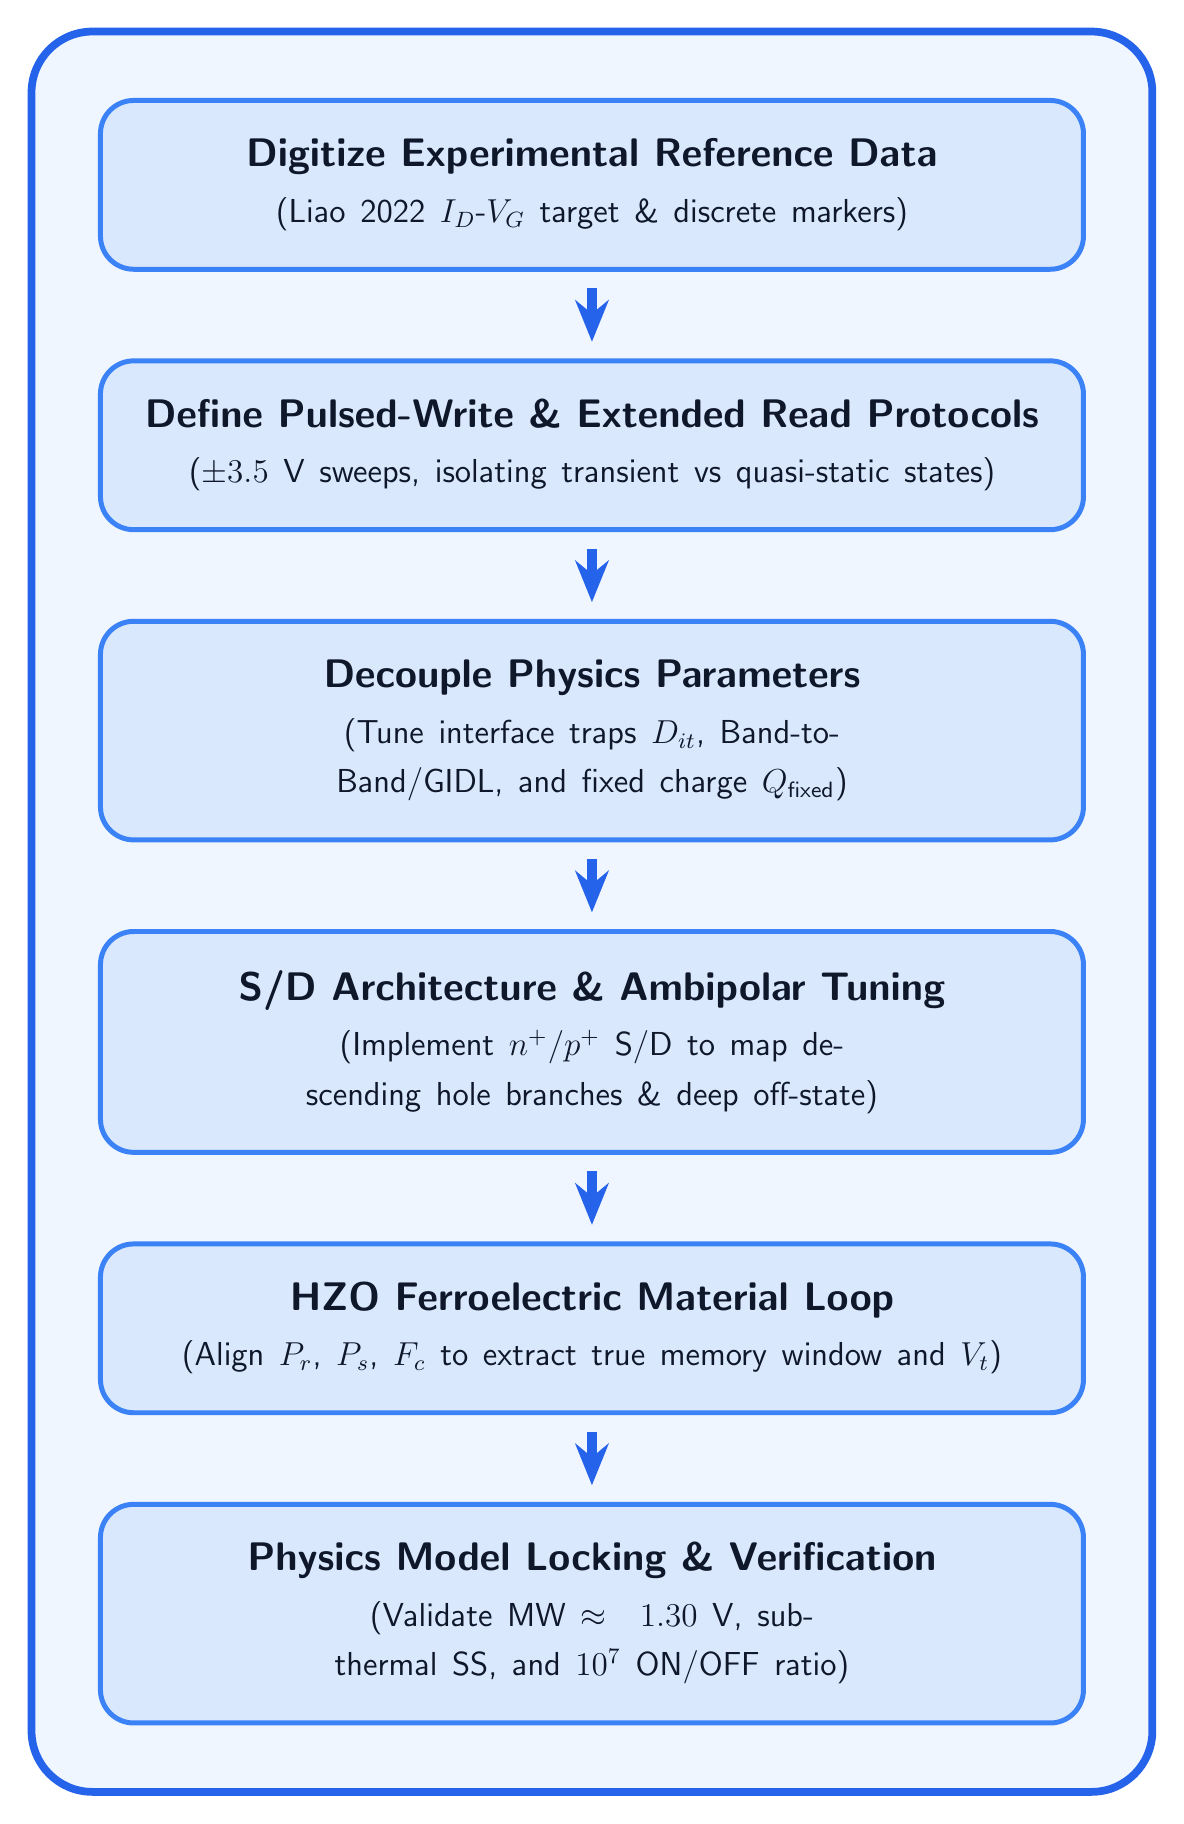
\begin{tikzpicture}[node distance=1.1cm]

  % Steps
  \node (s1) [stepbox] {Digitize Experimental Reference Data\\[2pt]{\large\normalfont(Liao 2022 $I_D\text{-}V_G$ target \& discrete markers)}};
  
  \node (s2) [stepbox, below=of s1] {Define Pulsed-Write \& Extended Read Protocols\\[2pt]{\large\normalfont($\pm3.5$ V sweeps, isolating transient vs quasi-static states)}};
  
  \node (s3) [stepbox, below=of s2] {Decouple Physics Parameters\\[2pt]{\large\normalfont(Tune interface traps $D_{it}$, Band-to-Band/GIDL, and fixed charge $Q_{\text{fixed}}$)}};
  
  \node (s4) [stepbox, below=of s3] {S/D Architecture \& Ambipolar Tuning\\[2pt]{\large\normalfont(Implement $n^+/p^+$ S/D to map descending hole branches \& deep off-state)}};
  
  \node (s5) [stepbox, below=of s4] {HZO Ferroelectric Material Loop\\[2pt]{\large\normalfont(Align $P_r$, $P_s$, $F_c$ to extract true memory window and $V_t$)}};
  
  \node (s6) [stepbox, below=of s5] {Physics Model Locking \& Verification\\[2pt]{\large\normalfont(Validate MW $\approx 1.30$ V, sub-thermal SS, and $10^7$ ON/OFF ratio)}};

  % Background container
  \begin{scope}[on background layer]
    \node (fitbox) [container, fit=(s1) (s2) (s3) (s4) (s5) (s6)] {};
  \end{scope}

  % Connectors
  \draw [flowarrow] (s1) -- (s2);
  \draw [flowarrow] (s2) -- (s3);
  \draw [flowarrow] (s3) -- (s4);
  \draw [flowarrow] (s4) -- (s5);
  \draw [flowarrow] (s5) -- (s6);

\end{tikzpicture}
\end{document}
